%% 研究報告用スイッチ
%% [techrep]
%%
%% 欧文表記無しのスイッチ(etitle,jkeyword,eabstract,ekeywordは任意)
%% [noauthor]
%%

\documentclass[submit,techrep]{ipsj}
%\documentclass[submit,techrep,noauthor]{ipsj}



\usepackage[dvips]{graphicx}
\usepackage{latexsym}
\usepackage[dvipdfmx]{}

\def\Underline{\setbox0\hbox\bgroup\let\\\endUnderline}
\def\endUnderline{\vphantom{y}\egroup\smash{\underline{\box0}}\\}
\def\|{\verb|}

\setcounter{巻数}{58}%vol53=2012
\setcounter{号数}{10}
\setcounter{page}{1}

\begin{document}


\title{マルチテナントシステムの開発を支援するIaaS環境}

\etitle{IaaS environment to support multi-tenant system development}

\author{古橋 健斗}{Kento Furuhashi}{Shibaura Institute of Technology}[ma17099@shibaura-it.ac.jp]
\author{松本 拓也}{Takuya Matsumoto}{Shibaura Institute of Technology}
\author{福田 浩章}{Hiroaki Fukuda}{Shibaura Institute of Technology}[hiroaki@shibaura-it.ac.jp]

\begin{abstract}
クラウドサービスでは,アプリケーションを提供するサービス提供者が物理マ
シンやネットワークを保有するインフラ提供者から必要に応じてリソース
(e.g., 仮想マシン)を確保し,サービスを提供している.サービス提供者は,
最大負荷(必要になる仮想マシンの最大数)を見積もることでサービスの円滑な
運用を目指しているが,予め見積もることは難しい.一方,インフラ提供者は,
物理マシン,仮想マシンの負荷状況(e.g, CPUやメモリ使用量)をもとに仮想マ
シンを再配置し,データセンタ全体の運用効率向上を目指している
.この検証には実運用に適用することが望ましい
が,サービス提供者のSLAを保証する必要があり,実現は難しい.また,大規
模なデータセンタを準備することも難しいため,シミュレーションでの検証を
行わざるをえない.そこで本研究では,RaspberryPIを利用し,
サービス提供者,インフラ提供者それぞれの要求を容易にテストできる環境を
提供する.具体的には,複数のRaspberryPIを使用した仮想データセンタの構
築と負荷状況の監視,仮想マシンの操作を実現する.また,必要に応じて仮想
マシンを増減し,スケールアウトする機能を実現する.そして,仮想マシンの
移動,スケールアウトを本環境で実行し,その機能性能を示す.
\end{abstract}

%
%\begin{jkeyword}
%情報処理学会論文誌ジャーナル,\LaTeX,スタイルファイル,べからず集
%\end{jkeyword}
%
%\begin{eabstract}
%This document is a guide to prepare a draft for submitting to IPSJ
%Journal, and the final camera-ready manuscript of a paper to appear in
%IPSJ Journal, using {\LaTeX} and special style files.  Since this
%document itself is produced with the style files, it will help you to
%refer its source file which is distributed with the style files.
%\end{eabstract}
%
%\begin{ekeyword}
%IPSJ Journal, \LaTeX, style files, ``Dos and Dont's'' list
%\end{ekeyword}

\maketitle

%1
\section{はじめに}
仮想化技術の進化を背景に,物理マシンを保有してサービスを展開する形態
(シングルテナント)から,必要に応じてリソース(e.g., CPUやメモリ)を確保
しサービスを展開する形態(マルチテナント)に移行している.そして,これら
はAmazon Web Service~(AWS)\cite{aws}やMicrosoft Azure\cite{azure}のようなクラウドサービスを利用して提供されている.マルチテナン
ト環境では,図\ref{fig:user}に示すようにアプリケーションを提供するサー
ビス提供者が物理マシンやネットワークを保有するインフラ提供者から必要に
応じてリソース(e.g., 仮想マシン)を確保し,サービスを提供している.サー
ビス提供者は,最大負荷(必要になる仮想マシンの最大数)を見積もることでサー
ビスの円滑な運用を試みるが,予め正確に見積もることは難しい.そのため,
実際には経験に基づき最大数を設定し,運用している.一方,インフラ提供者
は,物理マシン,仮想マシンの負荷状況(e.g, CPUやメモリ使用量)をもとに仮
想マシンを再配置し,データセンタ全体の運用効率向上を目指している
\cite{cloud1}\cite{cloud2}.この検証には実運用に適用することが望ましい
が,サービス提供者のService Level Agreement~(SLA)を保証する必要があり,実現は難しい.また,大規
模なデータセンタを準備することも難しいため,シミュレーションでの検証を
行わざるをえない\cite{testbed}.

一方,近年小型計算機の開発を背景に,それらを複数台利用してクラスタとし
て利用する事例や,SDNの検証に用いる例が見受けられる.小型計算機は一般
の計算機やサーバと比較して安価で,複数台用意することも十分に可能である.
また,仮想化機能を備えたCPUを搭載する小型計算機も存在する.

そこで本研究では,小型計算機の一つであるRaspberryPI(RasPI)を利用してデー
タセンタを模擬し,インフラ提供者が効率の良いデータセンターの運用方式
(e.g., アルゴリズム)を開発するテスト環境を提供する.また,予め最大数を
見積もることなく,物理マシン,仮想マシンの状況に応じて動的に仮想マシン
を複製し,動的に負荷を分散する機構(オンデマンドスケールアウト)を実現す
る.そして,負荷分散や運用効率を判定する指標となるCPUやネットワークの
負荷の取得する機能,および仮想マシンの複製や移動を実行する機能をAPIと
して提供する.最後に,これらのAPIを使用して仮想マシンの移動,スケール
アウトを実行し,テスト環境の基本性能を示す.

以降,2節では本研究で想定するクラウド環境について概説し,テスト環境の要件を整理する.
3節では本研究のアプローチについて概説し,4節で
実装について述べる.次に5節ではテスト環境での実験と結果をまとめる.
そして,6節で関連研究について述べ,最後7節でまとめと今後の課題を述べる.

\begin{figure}[tb]
	\includegraphics[width=8.5cm,bb=0 0 752 480]{fig/user.png}
	\caption{マルチテナント環境}
	\label{fig:user}
\end{figure}

\section{クラウド環境とテスト環境の要件}
本節では,本研究で想定するクラウド環境を概説し,それらの実現に必要なテスト環境の要件を述べる.
\begin{figure}[tb]
	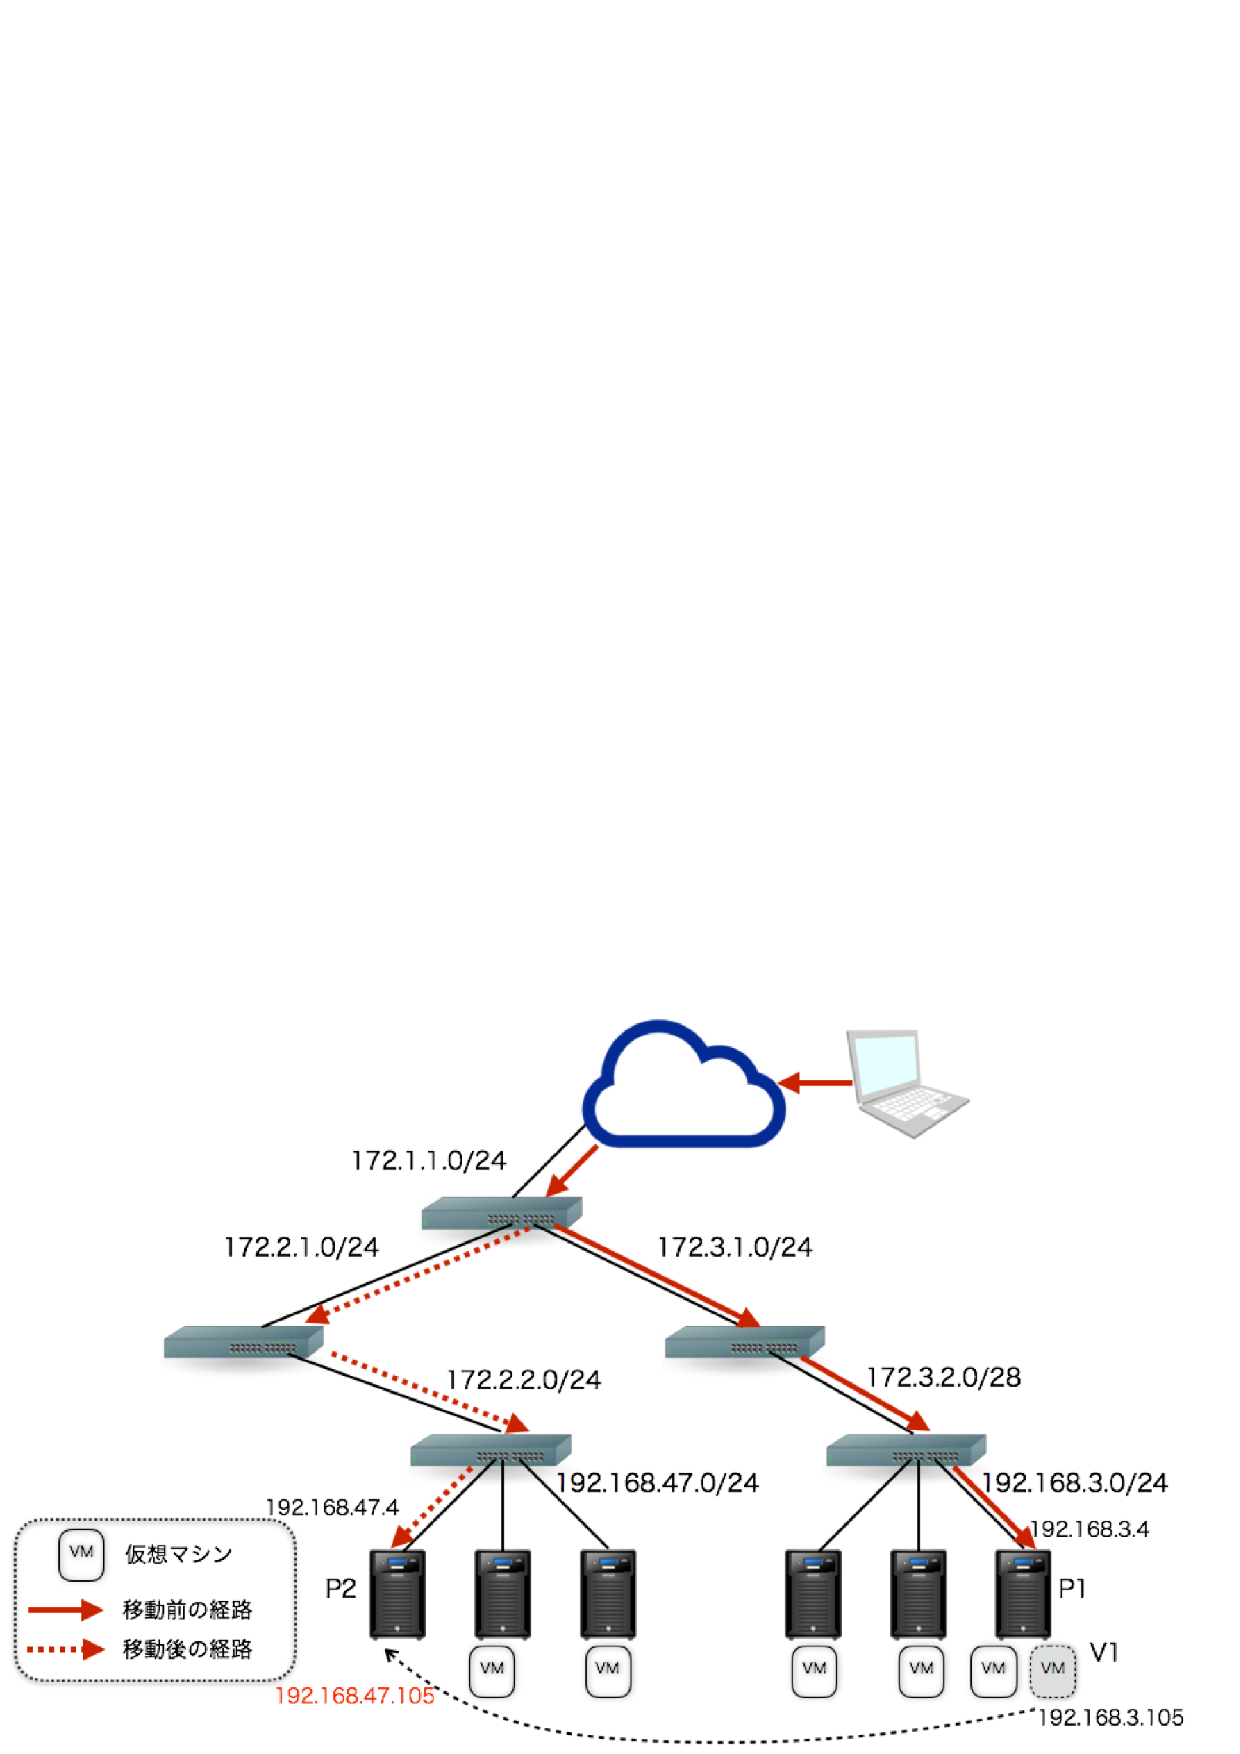
\includegraphics[width=8.5cm,bb=0 0 579 366]{fig/cloud.png}
	\caption{想定するクラウド環境}
	\label{fig:cloud}
\end{figure}

\subsection{クラウド環境}
\label{subsec:cloud}
本研究で想定するクラウド環境を図\ref{fig:cloud}に示す.クラウド環境で
は,一般に複数のネットワークスイッチとそれらに接続した物理マシンで構成
される.そして,サービス提供者からリソース取得の要求があると,インフラ
提供者は物理マシンで仮想マシンを起動してそれらを提供している.クライア
ントのリクエストはスイッチで適切に転送され,対象となる仮想マシンが適切
に処理してサービスを運用している.ここで,物理マシンが高負荷になり,仮
想マシンが移動する状況を想定する~(図\ref{fig:cloud}).図
\ref{fig:cloud}では,物理マシンP1で仮想マシンV1が動作している状況にお
いて,V1を物理マシンP2に移動することを想定している.P1とV1にはそれぞれ
IPアドレス(192.168.3.4, 192.168.3.105)が設定されており,ユーザの立場か
らは区別できない.一方,P2にも192.168.47.4のIPアドレスが設定されている.
仮想マシンの移動では,一般にIPアドレスは変化しないため,V1のIPアドレス
はP2に移動した後も変わらず192.168.3.105となる.V1の移動はP2が直接接続
しているネットワークスイッチ,および上流に位置するスイッチに影響しない
ため,従来V1に届けられていたパケットは依然として192.168.3.0/24を管理す
るスイッチに届けられることになり,移動後のV1に届けられることはない.移
動後のV1に正しくパケットを届けるためには,V1のIPアドレスと移動後のネッ
トワークに合致したものに変更(e.g., 192.168.47.105)する必要がある.しか
しながら,ユーザがこの変更を知る手段がないため,V1へのリクエストは依然
として192.168.3.105宛に送信される.したがって,リクエストを正しく移動
後のV1に届けるためには,ネットワークスイッチに変更を加え,宛先
192.168.3.105へのパケットは変更後のアドレス(192.168.47.105)に書き換え
る必要がある.

このように,クラウド環境で円滑にサービスを運用するためには,仮想マシンの移動や
複製に伴い,関連するネットワークスイッチも連動して変更する必要がある.

\subsection{テスト環境の要件}\label{subsec:requirement}
\ref{subsec:cloud}節で述べたように,本研究で想定するクラウド環境の実現
には,仮想マシンの移動だけでなく,IPアドレスの変更など,移動に伴う変更
や,移動の契機となる状況の把握,多数のマシンを制御する必要がある.そこ
で本研究では,クラウド環境を実現するため,以下の項目をクラウド環境の必
要要件と考える.

\begin{description}
\item [負荷状況の把握]仮想マシンの移動や複製は,一般に高負荷状態にある
  物理マシンの負荷を分散し,仮想マシンで提供するサービスの性能維持や,
  低負荷状態の物理マシンに散財する仮想マシンを集約し,リソースの効率的
  な使用のために行われる.本テスト環境でもこれらの負荷状態を測定する
  ため,負荷状態の判定に一般的に用いられるCPUとメモリ使用率を使用する.
  また,物理マシンの負荷分散を目的として仮想マシンを移動させる場合,移
  動先物理マシンを決定する必要があるが,主としてネットワークを利用したサービス
  に用いられるクラウド環境ではネットワーク使用量も移動先を決定する
  指標となり得る.そこで本研究では,物理マシン単体のネットワーク使用量
  だけでなく,スイッチ単位でのネットワーク使用量を測定し,移動先決定の
  指標に用いる.

\item [IPアドレスとルーティング管理]仮想マシンが移動する時,移動先物理マシンが同一
  ネットワークに所属している場合にはIPアドレスの変更は必要ない.しかし,
  \ref{subsec:cloud}節でも述べたように,異なるネットワークに所属する物
  理マシンに移動する場合には移動後にIPアドレスの変更が必要になる.同一
  ネットワーク内だけの移動/複製は,クラウド環境の効率的な運用の妨げに
  なるため,本研究ではネットワーク間を跨いだ仮想マシンの移動/複製も想定
  する.その場合,複数の物理/仮想マシンに同一のIPアドレスを指定するこ
  とはできないため,仮想マシン移動時にはIPアドレスを開放し,移動後には
  未使用のIPアドレスを設定する必要がある.
  さらに,ネットワーク間を跨いだ仮想マシンの移動/複製には,\ref{subsec:cloud}節で述べたように,
  IPアドレスの変更に伴い,関連するネットワークスイッチを変更し,適切にクライアントからのリクエストを
  転送する必要がある.

\item [複数マシンの管理]本研究では,クラウド環境の効率的な運用のため,
  仮想マシンの移動/複製を効率的に行うアルゴリズム開発/検証にテスト環境
  を利用することを想定している.そのため,本テスト環境は多数の物理マシ
  ン,ネットワークスイッチで構成することになり,それぞれの状態管理
  (e.g, 負荷の測定)や制御(e.g, 設定変更や仮想マシンの移動/複製)を個別
  に行うことは現実的に難しい.そこで,テスト環境を構成する物理マシン
  やネットワークスイッチを一元管理し,設定変更や制御を用意に実現できる
  必要がある.

\end{description}

\section{テスト環境の実現}
本節では,RasPIで仮想環境を実現する方法について述べた後,
\ref{subsec:requirement}節で挙げた要件に対応する本研究での実現方法を述
べる.

\begin{table}[tb]
	\centering
	\caption{RaspberryPi2 ModelBの性能}
	\label{tab:rpi2}
	{
		\small
		\begin{tabular}{|c|c|} \hline
		CPU & ARM Cortex-A7 クアッドコア 900MHz\\ \hline
		メモリ & 1GB\\ \hline
		ネットワーク & 10/100Mbpsイーサネット\\ \hline
		電源 & 900mA(4.5 \textasciitilde 5.5W)\\ \hline
		\end{tabular}
	}
\end{table}

\begin{table}[tb]
	\centering
	\caption{QEMUの機能}
	\label{tab:qemu_func}
	{
		\small
		\begin{tabular}{|c|c|} \hline
		qemu-img & 仮想マシンのイメージファイルの作成\\ \hline
		qemu-system-arm & 仮想マシンの起動\\ \hline
		migrate & 仮想マシンの移動\\ \hline
		\end{tabular}
	}
\end{table}

\subsection{RaspberryPIでの仮想化環境}
本研究のテスト環境では表\ref{tab:rpi2}に示すRaspberryPI2 ModelBを利用し,
Linux系専用OSであるRaspbian Jessie Lite\cite{raspbian}を実行する.CPUであるARM
Cortex-A7は仮想化拡張機能を備えているため,Linuxカーネルが備えるハイパー
バイザ,KVMを実行することができる.一般のPCでは,KVMはパッケージ管理ソ
フトウェア(e.g., apt-get)などを利用してインストールできるが,RasPIでは
パッケージでは提供されていない.そのため,カーネルの組み込み機能として
実行する.また,KVMでの仮想マシンの管理にはvirt\cite{virt}を利用することが
一般的であるが,RasPIではvirtを利用することができない\footnote{インストールは可能であるが,
実行できない}.そのため,本研
究ではKVMと連携して動作するqemu\cite{qemu}が提供する機能(表\ref{tab:qemu_func})を利用する.

一方,\ref{subsec:requirement}節でも述べたように,本テスト環境の実現に
は仮想マシンの移動/複製に同期したネットワークの変更が必要になる.近年,
仮想化技術の進歩に伴い,ネットワークを柔軟に制御するためにSoftware
Defined Network~(SDN)\cite{sdn}が注目を集めており,利用されている.そ
こで本研究でもSDNを利用してネットワークを制御する.本研究ではSDNの一種
であり,広く利用されているOpenFlow\cite{opf}を利用するため,OpenFlow対
応のソフトウェアスイッチであるOpen vSwitch(OvS)をRasPIにインストールし
て利用する.そのため,本テスト環境はすべてRasPIだけで構成できる.

\begin{figure}[tb]
	\includegraphics[width=8.0cm,bb=0 0 815 574]{fig/topology.png}
	\caption{テスト環境のトポロジ}
	\label{fig:topology}
\end{figure}

\subsection{OpenFlowの概要}
SDNでは,経路制御を行うコントロールプレーンとデータの転送を行うデータ
プレーンが共存する既存のネットワーク機器とは異なり,コントロールプレー
ンとデータプレーンを分離したアーキテクチャを採用している.OpenFlowで
は,データプレーンをOpenFlowスイッチと呼び,OpenFlowスイッチを制御す
るコントロールプレーンをOpenFlowController(OFC)と呼ぶ.  OpenFlowスイッ
チではデータの転送のみを行い,経路制御は OFCによって行われる.
OpenFlowスイッチは,パケットが内包する情報(送信元/送信先IPアドレスなど)を条件に
対象となるパケットを抽出し,それらに対して適切なアクション(パケット転送など)を実行する.
この,条件とアクションの組み合わせをフローと呼び,それらをまとめたテーブルをフローテーブルと呼ぶ.
OpenFlowスイッチはフローテーブルを保持し,自身がもつフローに従ってパケットを処理する.そして,
条件に合致しないパケットをOpenFlowが受信した場合,OpenFlowスイッチはOFCに問い合わせ(パケットイン),
適切なフローを受信してパケットを処理すると伴に,フローテーブルに記憶する.

%OpenFlowでは,OpenFlowスイッチにパケットが到達すると,OpenFlowスイッチが保持するフローテーブルを確認する.
%OpenFlowスイッチはフローテーブルに記述されているフローに従い受け取ったパケットの転送を行う.
%フローテーブルにフローが記述されていれば,フローに従い転送を行うが,記述されてない場合には,OFCに制御ルールの問い合わせを行う.
%問い合わせを受けたOFCはOpenFlowスイッチにフローを返す.
%制御ルールを受け取ったOpenFlowスイッチはフローテーブルにフローを追加し,その フローに従いパケットを宛先まで転送を行う.

\subsection{テスト環境のアーキテクチャ}\label{subsec:arch}
\ref{subsec:requirement}節で述べたように,多数の物理マシンや仮想マシンの
状態管理,および制御を個別に行うことは困難である.そこで,本研究では,
仮想マシンや仮想マシンを起動する物理マシンを一元管理する仮想マシンコン
トローラ(VMC)を実現する.また,KVMを用いた仮想マシンの移動にはNFSを利
用する必要があり,一般にNFSの利用はローカルネットワークであることが望
ましい.そこで本テスト環境では,図\ref{fig:topology}に示すように,ユー
ザがサービス利用のために利用するネットワークとは異なる管理ネットワーク
を設け,すべての物理マシンを管理ネットワークにも接続する.そして,この
管理ネットワークにVMCを接続することで,後述する負荷状況やIPアドレス,
およびルーティングの管理を容易にする.

\begin{table}[htb]
	\centering
	\caption{統計情報\cite{opf}}
	\label{tab:counters}
	\vspace{3mm}
	{
		\begin{tabular}{|l|c|} \hline
		カウンター & Bits \\ \hline \hline
		\multicolumn{2}{|c|}{フローテーブルごと} \\ \hline
    有効エントリー数 & 32 \\
    パケットルックアップ数 & 64 \\
    パケットマッチ数 & 64 \\ \hline
		\multicolumn{2}{|c|}{フローごと}\\ \hline
    受信パケット数 & 64 \\
    受信バイト数 & 64 \\
    フローが作られてからの経過時間(秒) & 32 \\
    フローが作られてからの経過時間(ナノ秒) & 32 \\ \hline
		\multicolumn{2}{|c|}{ポートごと} \\ \hline
    受信パケット数 & 64 \\
    転送パケット数 & 64 \\
    受信バイト数 & 64 \\
    転送バイト数 & 64 \\
    受信ドロップ数& 64 \\
    転送ドロップ数& 64 \\
    受信エラー数 & 64 \\
    受信フレームアライメントエラー数 & 64 \\
    受信オーバーランエラー数 & 64 \\
    受信CRCエラー数 & 64 \\
    コリジョン数 & 64 \\ \hline
    \multicolumn{2}{|c|}{キューごと} \\ \hline
    転送パケット数 & 64 \\
    転送バイト数 & 64 \\
    転送オーバーランエラー数 & 64 \\ \hline
		\end{tabular}
	}
\end{table}

\subsection{負荷状況の把握}
負荷状況の指標となる各物理マシンのCPUとメモリ使用率,各スイッチのトラ
フィック量を取得する.CPUとメモリ使用率の取得には,各物理マシンの/proc
ディレクトリ以下に格納される情報(meminfo)を利用し,一定間隔(現在は10
秒)で継続的に取得する.また,トラフィック量の取得には,表
\ref{tab:counters}で示すOvSが保持する統計情報を利用し,各OvS単位,およ
び個々のOvSのポート単位でのトラフィック量を計測する.これらの情報を
OFCに集約し,これらの情報を取得するAPIを提供す
ることでVMCと連携する.

\subsection{IPアドレスとルーティング管理}
\label{subsec:ip_routing}
%IPアドレスは自前で管理する
%移動:
%同一ネットワークではなにもしない
%ネットワークをまたぐ場合:()IPの変更,ルーティングテーブルの変更
%複製:
%ラウンドロビン.変更するスイッチの特定
\ref{subsec:cloud}節で述べたように,クラウド環境の実現には仮想マシンの
移動や複製だけでなく,関連するネットワークスイッチも連動して変更する必
要がある.そのため,本テスト環境では仮想マシンに使用するIPアドレスは
DHCPを用いることなくVMCが管理し,仮想マシンの移動に同期した変更を可能
にする.本テスト環境では,仮想マシンに付与するIPアドレスのネットワーク
アドレスは,物理マシン所属するネットワークアドレスと同一である必要があ
る.そのため,移動や複製に伴い変更の必要がある.本テスト環境では,使用
中のIPアドレス,ネットワークアドレスをVMCで集中管理しており,仮想マシ
ンの移動や複製先のネットワークに適したIPアドレスを付与する.仮想マシン
への具体的な設定は,ifconfigやrouteコマンドを使用したスクリプトを用意
している.

次に,\ref{subsec:cloud}節で述べたように,クライアントのリクエストを正
しく移動,または複製後の仮想マシンに届けるためには,リクエストを経由す
るスイッチを適切に変更する必要がある.
VMCは仮想マシンの移動または複製を行った後,移動・複製前,および
移動・複製後のIPアドレス,実行の種類(移動または複製)をOFCに通知する.
OFCは関連するOvSを特定し,適切に設定変更する必要がある.
以降,同一ネットワーク,およびネットワークを跨いで仮想マシンが
移動または複製されるときの設定変更について述べ,最後に関連するOvSの特
定について述べる.


%テスト環境では,使用中のIPアドレスをVMCで動作するデータベースで管理し,仮想マシンの
%起動や複製,移動時に次の手順で決定し,実際に設定する.
%まず,移動先物理マシンが所属するネットワークアドレスを調べ,使用中のIPアドレス一覧を
%取得する.次に,ネットワークアドレス,ブロードキャストアドレス,使用中のIPアドレスを
%除きランダムで決定しする.最後に,起動,複製,移動後の仮想マシンのifconfig,route
%コマンドを使用してIPアドレスとデフォルトルートを設定する.

%次に,異なるネットワークに仮想マシンの移動や複製を行う場合,OpenFlowを
%利用し,経由するOvSの設定を変更することで,パケットの転送経路を変更す
%る.具体的には,仮想マシンを移動する時,OFCはすべてのOvSのルーティング
%情報を保持ししているため,移動前アドレスのルーティングテーブルが存在す
%るOvSを探索し,パケットを転送するポートを変更すると同時にパケットの送
%信先アドレスを変更する.そして,移動後の仮想マシンから戻るパケットに関
%しては,送信元アドレスを移動前のアドレスに書き換えて送信する.また,仮
%想マシンを複製する時には,移動と同様の処理を1/2の割合で実行すること
%により,ラウンドロビンで負荷を分散する.

\begin{figure}[tb]
	\includegraphics[width=8.5cm,bb=0 0 872 468]{fig/migrate_flow.png}
	\caption{同一ネットワークへの仮想マシンの移動}
	\label{fig:migrate_flow}
\end{figure}
\begin{figure}[tb]
	\includegraphics[width=8.5cm,bb=0 0 958 401]{fig/migrate_flow_diff.png}
	\caption{外部ネットワークへの仮想マシンの移動}
	\label{fig:migrate_flow_diff}
\end{figure}
\begin{figure}[tb]
	\includegraphics[width=8.5cm,bb=0 0 955 468]{fig/clone_flow.png}
	\caption{仮想マシンの複製}
	\label{fig:clone_flow}
\end{figure}

%次に仮想マシンの移動,複製時のOpenFlowの動作を説明する.
%VMCから仮想マシンの移動/複製の命令を受け取ったOFCは,接続されている全てのOvSのフローテーブルを取得する.
%フローテーブルの解析を行い,これらの仮想マシンの移動/複製を行なった時にフローが分岐するスイッチを特定し,そのスイッチにフローテーブルの書き込みを行う.
%フローテーブルの書き込みの時,VMCからは移動/複製元の仮想マシンのIPアドレスと移動/複製先の仮想マシンのIPアドレスが通知される.

\begin{enumerate}
 \item 同一ネットワークへの仮想マシンの移動\\同一ネットワーク内の仮想
   マシンの移動ではIPアドレスの変更は行われない.したがって,図
   \ref{fig:migrate_flow}に示すように,特定したOvSにおいて,転送先アド
   レスがVM1(192.168.1.10)にマッチしたパケットの送出ポート番号を変更す
   る(Port2 $\rightarrow$ Port3).


 \item 外部ネットワークへの仮想マシンの移動\\外部ネットワークへの仮想
   マシンの移動では,IPアドレスの変更が伴う.図
   \ref{fig:migrate_flow_diff}では,異なるネットワークに所属するPM1と
   PM2間で仮想マシンが移動する.そこで,OvSでは転送先アドレス
   192.168.1.10にマッチしたパケットの送出ポートを変更し(Port2
   $\rightarrow$ Port3),かつパケットのDSTアドレスを変更する
   (192.168.1.10 $\rightarrow$ 172.168.1.10).さらに,172.168.1.10から
   の送信元に戻されるパケットについては,OvSでSRCアドレスを
   192.168.1.10に書き換える.その結果,クライアントが仮想マシンの移動
   に気づくことはない.

%\item 仮想マシンの移動\\
%仮想マシンを移動する時,移動元仮想マシンへパケットを転送するフローは参照されなくなる.
%図\ref{fig:migrate_flow}の例では,VM1へ転送を行おうとした場合に,VM2に転送されるので,VM1へは転送されない.
%しかし,VM1への転送を行うフローは参照されないので,こういったフローがたまることでOvSの性能を下げてしまう.
%そこで,以上のフローテーブルの書き込みが終了した時,VM1へ転送を行うフローの削除を行う.

 \item 仮想マシンの複製\\仮想マシンが複製される場合,同一ネットワーク
   か否かに関わらず,複製した仮想マシンには新たなIPアドレスが割り当て
   られ,仮想マシン間でリクエストを分散して処理する.このとき,複製前
   に既にリクエストを処理したクライアントに対しては複製前の仮想マシン
   がリクエストを処理し,新たにリクエストを送信したクライアントに関し
   てはラウンドロビンで処理を分散する.

   図\ref{fig:clone_flow}は2台のクライアント(IP1, IP2)のうちIP1が
   VM1(192.168.1.10)に既にアクセスしており,VM2(192.168.1.20)を生成後,
   IP2がVM1に対してリクエストを送信したときの様子を示している.IP1から
   VM1へのリクエストは既に実行されているため,IP1からVM1へのリクエスト
   はOvSのフローテーブルに従って引き続きPort2に送出される.一方,IP2か
   らVM1へのリクエストはOvSのフローテーブルにマッチしないため,OvSは
   OFCに処理の問い合わせを行う(パケットイン).この時,OvSはVMCによって
   複製されたVM2のIPアドレスを認識しているため,パケットのDSTアドレス
   を変更する(192.168.1.10 $\rightarrow$ 192.168.1.20)してPort3に送出
   する.そして,学部ネットワークへ仮想マシンの移動と同様,戻りパケッ
   トのSRCアドレスをVM1のものに書き換える(192.168.1.10).
   その結果,処理の分散はクライアントには透過であり,既存のクライアント(IP1)
   のセッションも維持される.

\end{enumerate}

\begin{table}[tb]
	\centering
	\caption{使用できる機能}
	\label{tab:vmc_func}
	{
		\small
		\begin{tabular}{|l|l|} \hline
		仮想マシンの起動 & hostname/startVm/id\\ \hline
		複製 & hostname/clone/src\_id/dst\_id\\ \hline
		移動 & hostname/migrate/src\_id/dst\_id\\ \hline
		リソースの取得 & hostname/getResource\\ \hline
		\end{tabular}
	}
\end{table}

\subsection{複数マシンの管理}
\ref{subsec:arch}で述べた通り,VMCを使用することで,多数の物理マシンや仮想マシンの状態管理や制御を個別に行うことが可能になる.
本テスト環境の利用者は,WebAPIを利用することによって,各物理マシンの操作を行うことができる.
VMCを起動すると,自動的にサーバが起動する.
本システムの利用者はそのサーバにアクセスすることで表\ref{tab:vmc_func}に示す機能を使用できる.
各物理マシン,仮想マシンのIDやリソース状況はhostname/indexで確認することができる.
仮想マシンの起動には仮想マシンを起動する物理マシンのIDを指定する.
仮想マシンの複製には,複製する仮想マシンのIDと複製先の物理マシンのIDを指定する.
仮想マシンの移動には,移動する仮想マシンのIDと移動先の物理マシンのIDを指定する.
リソースの取得は全ての物理マシン,仮想マシンのリソース情報がJSON形式でデータが渡される.
また,IDを指定することで指定したマシンのリソースの取得も行うことができる.
このWebAPIを使用することで,仮想マシンの起動,移動,複製と各物理マシンのリソースの取得を行えるので,アルゴリズムのテストを行うことができる.

\section{評価}
本節では,RasPI 17台(OvSに7台,PMに8台,OFCとVMCにそれぞれ1台)を使用し
て図\ref{fig:topology}に示すトポロジを構成し,本テスト環境を評価する.

まず,RasPIでのOpenFlow環境が十分な性能を有すること
を示すため,複数のOvSを経由するときのトラフィック量を計測し,スループッ
トを示す.次に,仮想マシンの移動,および複製時の実行時間を測定して
本テスト環境の基本性能を示す.最後に,仮想マシンの移動,複製時,時間経
過に伴うのCPUとメモリ使用率を測定し,考察する.


\begin{table}[tb]
	\centering
	\caption{サーバを通信する時の経由するOvSの数}
	\label{tab:route}
	\vspace{4mm}
	{
		\begin{tabular}{ c c c } \hline
      route & 通信間 & 経由するOvS数 \\ \hline \hline
      1 & PM1 $\longleftrightarrow$	PM2 & 1 \\ \hline
      2 & Internet $\longleftrightarrow$ PM1 & 3 \\ \hline
      3 & PM1 $\longleftrightarrow$	PM3 & 3 \\ \hline
      4 & PM1 $\longleftrightarrow$	PM8 & 5 \\ \hline
		\end{tabular}
	}
\end{table}

\begin{figure}[tb]
	\includegraphics[width=8.5cm,bb=0 0 755 558]{fig/graph.png}
	\caption{ネットワーク速度}
	\label{fig:graph}
\end{figure}

\subsection{RasPIでのOpenFlow環境}
RasPIを用いたOvSのスループットを測定するため,図\ref{fig:topology}に示
すトポロジにおいて,表\ref{tab:route}に示す経路でネットワークに負荷を
かけ,スループットを計測する.この計測にはiperf\cite{iperf}を利用し,
最大TCPセグメントを,128/256/512/1024/1400[Byte]としたときの値を測定し
た.まず,設定した最大TCPセグメントに依存せず,route1とroute4を比較す
ると分かるように,経由するOvSの数によって僅かに転送速度が低下する.こ
れは,パケット転送に関連するOvSの個数の影響であり,最大でも5Mbps程度の
性能低下であることから(最大TCPセグメントサイズ1024[Byte]の場合),極端
な速度低下は見られない.
また,最大TCPセグメントサイズを2倍にするごとににスループットも倍増していることから,
パケット転送に関しては十分な性能が得られていることがわかる.なお,最大TCPセグメントサイズ
が1400[Byte]の場合,1024[Byte]の場合と比較して大幅なスループットの向上は見られなれなかった.
これは,RasPIのイーサネットポートが10/100Mbps対応であり,100Mbps以上のスループットを得られないためである.
一方,各OvSでは表\ref{tab:counters}で示した情報を取得できるため,本研究で実装したトラフィック取得機能を用いて
関連するOvSのトラフィック量を計測した.その結果,計測したトラフィック量の合計がiperfで転送したトラフィック量と
一致することを確認した.

これらの結果から,RasPIでのOpenFlow環境は十分な性能が得られると判断することができる.

\begin{table}[tb]
	\centering
	\caption{仮想マシンの操作に要する時間}
	\label{tab:func_time}
	\vspace{4mm}
    \scalebox{1.0}
	{
		\begin{tabular}{|c|c|c|c|} \hline
            仮想マシンの操作& 起動(秒) & 移動(秒) & 複製(秒) \\ \hline \hline
            実行時間 & 47 & 32 & 49 \\ \hline
            ネットワーク構成変更 & & 3 & 4 \\ \hline
	  	\end{tabular}
	}
\end{table}

\begin{table}[tb]
	\centering
	\caption{表\ref{tab:func_time}の実行時間内訳}
	\label{tab:func_breakdown}
	\vspace{4mm}
    \scalebox{1.0}
	{
		\begin{tabular}{|c|c|c|c|} \hline
            仮想マシンの操作& 起動(秒) & 移動(秒) & 複製(秒) \\ \hline \hline
						Qemuの機能 & 32 & 23 & 32 \\ \hline
						スナップショットの転送 & - & 2 & 2 \\ \hline
						ネットワークの設定 & 8 & - & 8 \\ \hline
						リソースの取得 & 7 & 7 & 7 \\ \hline
            合計 & 47 & 32 & 49 \\ \hline
	  	\end{tabular}
	}
\end{table}

\subsection{仮想マシンの移動と複製}
\label{subsec:migrate_duplicate}
本テスト環境では,仮想マシンの起動にqemuのスナップショット機能
\cite{snapshot}を用いている.また,この機能は仮想マシンの複製時にも利
用する.そのため,仮想マシンの移動と複製に加え,スナップショットを用い
た起動時間を表\ref{tab:func_time}に示し,その内訳を表
\ref{tab:func_breakdown}に示す.

表\ref{tab:func_breakdown}に示すように,仮想マシンの起動は,$a$)スナッ
プショットファイルを指定したqemu-system-armコマンドの実行,
$c$)ifconfigやrouteコマンドを利用した,ネットワーク設定用スクリプト
の実行(ネットワークの設定),$d$)仮想マシンのリソース使用量を測定するスクリプトの実行(リソースの取得),
で構成される.表\ref{tab:func_breakdown}より,仮想マシンの起動には$a$)
に32秒,$c$)に8秒,$d$)に7秒要し,起動して使用可能になるまでに約47秒か
かった.一方,仮想マシンの移動には,$a'$)migrateコマンドの実行,$b$)ス
ナップショットの転送,$d$)リソースの取得,で構成され,$a'$)に23秒,$b$)
に2秒,$d$)に7秒要し,移動全体で32秒要した.なお,この実験では仮想マシ
ンは同一ネットワーク内を移動したため,$c$)ネットワークの設定は必要ない.

最後に,仮想マシンの転送は,仮想マシンの起動に加えスナップショットの転送が加わるため,
$a$), $c$), $d$)の実行に加え,b)スナップショットの転送に2秒要し,全体で49秒要した.

これら3つの結果から,起動や移動で用いるコマンドの違いによって$a$)と$a'$)で
は必要な時間が異なるが,$b$), $c$), $d$)に要する時間はどの場合でも同じ値を示
した.これらのことから,本テスト環境で実現した機能($b$), $c$), $d$))は,安定
して動作すると考えることができる\footnote{VMCやOFCと各PM間の通信,およびスナップショット転送は
管理ネットワークを使用するため,安定したスループットを得られる.}.

一方,\ref{subsec:ip_routing}節で述べたように,仮想マシンの移動と複製
には,VMCがそれらの完了を検知した後,OFCに依頼して関連するOvSを変更す
る,というネットワーク構成変更を伴う.したがって,表
\ref{tab:func_time}に示すように,仮想マシン移動時にはネットワーク構
成変更に伴いクライアントのリクエストが3秒間遮断されたが,複製では遮
断されることなく通信することができた.これは,仮想マシン移動時は構成変
更が終わるまでパケットを受け取る仮想マシンが存在しなくなるのに対し,仮
想マシンの複製では複製後の仮想マシンに関するネットワークの変更が行われ
るまでは複製元の仮想マシンにリクエストが届けられていることを意味してい
る.

この結果から,本テスト環境で提供するネットワーク構成変更は正しく機能していると推察される.


%本テスト環境の評価に先立ち,まずは仮想マシン操作についての評価を行う.
%はじめに仮想マシンの起動,複製,移動にかかった時間を計測した.
%その結果を表\ref{tab:func_time}に示す.
%仮想マシンの起動には約47秒かかった.
%その内訳を表に示す.
%仮想マシンの起動にはQEMUの機能を使用したが,QEMUの仮想マシンを起動するコマンドの実行時間は約30秒かかった.
%本研究での仮想マシンの起動にはIPアドレスの決定,設定,移動の時に使用するポート番号の決定を行う.
%また,テストのためにApacheを起動した.
%Apacheの起動には約40秒かかった.
%Apacheの起動を行う時,仮想マシンの起動には90.56秒かかった.
%次に仮想マシンの移動と複製の評価だが,これらにかかった時間はスイッチの経由数に関わらず一定であった.
%理由として,スイッチを経由せずにVMCを経由して転送や処理が行われたためである.
%実際に,OFCにはパケットの通知が行われなかった.
%VMCとPMはプライベートネットワークを設定しており,スイッチやユーザから見えるIPアドレスとは別のIPアドレスを設定しているのが原因であると推測した.
%これにより,時間の短縮とスイッチを経由するネットワークトラフィックの削減が見込めるため,弊害はないと考える.
%仮想マシンの移動には約32秒かかった.
%仮想マシンの移動ではイメージファイルの転送,待機状態の仮想マシンの起動,QEMUの機能による仮想マシンの移動を行う.
%QEMUの機能による仮想マシンの移動には約23秒の時間がかかった.
%また,仮想マシンの複製には約49秒かかった.
%仮想マシンの複製ではイメージファイルの転送,仮想マシンの起動を行う.
%仮想マシンの起動には47秒かかることがわかっているので,イメージファイルの転送に約2秒かかったことがわかる.
%\begin{table}[tb]
%	\centering
%	\caption{高性能物理マシンでの実行時間}
%	\label{tab:high_paformance_machine}
%	\vspace{6mm}
%    \scalebox{1.0}
%	{
%		\begin{tabular}{|c|c|c|} \hline
%            & 移動 & 複製  \\ \hline
%            実行時間 & 2.23秒 & 6.01秒\\ \hline
%		\end{tabular}
%	}
%\end{table}

%次に仮想マシンの移動と複製を,ネットワーク転送速度が1GBであり,IntelCore2DuoであるCPUを搭載した高性能物理マシンで実行し,その比較を行った.
%その結果を表\ref{tab:high_paformance_machine}に示す.
%この高性能物理マシンのCPU性能とネットワーク速度は本研究で使用するRasPI(性能は表\ref{tab:rpi2})の約10倍である.
%仮想マシンの移動には約14分の1,仮想マシンの複製は約8分の1の時間で処理が完了した.
%性能差と処理時間が比例していると考えると,仮想マシンの移動には時間がかかり,仮想マシンの複製には時間が短縮されたという結果となった.
%しかし,本研究の仮想マシンの移動,複製にはIPアドレスの決定や操作,ルーティングテーブルの決定などがあり,また,イメージファイルの転送にはスナップショットを用いているため,高性能物理マシンで実行した時と比較するとイメージファイルの転送量はきわめて少なくなっている.
%そのため,仮想マシンの移動ではIPアドレスの操作やQEMUに接続するなどの処理を行うため,時間がかかり,仮想マシンの複製ではスナップショットを使用したことにより処理時間が少なくなったと考えられる.
%また,仮想マシンの移動の時にも述べたが,QEMUの機能による仮想マシン移動コマンド単体の処理は23秒で処理が完了した.
%つまり,仮想マシンの移動だけを考慮すると,実行時間は10分の1になっていると考えられる.
%これにより,本環境で仮想マシンを操作した時の実行時間から,実際の環境で仮想マシンを操作した時のおよその実行時間を計算することができる.
%よって,本研究で実装した仮想マシンの操作は正常に行われ,実行時間は妥当であり,本テスト環境の値から実際の環境でかかるおよその時間を計測することができるので,本機能は十分使用できる性能だと言える.

%\begin{table}[tb]
%	\centering
%	\caption{サーバを通信する時の経由するOvSの数}
%	\label{tab:route}
%	\vspace{4mm}
%	{
%		\begin{tabular}{ c c c } \hline
%      route & 通信間 & 経由するOvS数 \\ \hline \hline
%      1 & PM1 $\longleftrightarrow$	PM2 & 1 \\ \hline
%      2 & Internet $\longleftrightarrow$ PM1 & 3 \\ \hline
%      3 & PM1 $\longleftrightarrow$	PM3 & 3 \\ \hline
%      4 & PM1 $\longleftrightarrow$	PM8 & 5 \\ \hline
%		\end{tabular}
%	}
%\end{table}
%\subsection{ネットワークの評価}
%次にネットワークの評価を行う.
%仮想マシンの複製や移動が発生した場合のルーティングが行われるまでの転送時間をiperf\cite{iperf}を用いて計測した.
%最大TCPセグメントサイズを128Byte/256Byte/512Byte/1024Byte/1400Byteの5段階に設定し,表\ref{tab:route}に示す状況においてそれぞれ計測した.
%表\ref{tab:route}のPMは図\ref{fig:topology}のPMを指している.
%仮想マシンの移動を実際に行うと,仮想マシンの移動の発生から完了,その後にネットワーク構成変更まで平均して合計約38秒かかった.
%p仮想マシンの移動の実験には,図\ref{fig:topology}の環境で1つのスイッチを経由するルートで行なった.
%仮想マシンの移動を行うと,表\ref{tab:func_time}のような結果になった.
%仮想マシンの移動の開始から完了するまでは,移動元の仮想マシンが動作中であるため,ネットワークが切れることはなく,仮想マシンの移動の完了後,移動元の仮想マシンが停止し,ネットワークの構成変更時に初めてネットワークが遮断される.
%実験の結果,ネットワークの構成変更には約3秒かかる事が結果として得られている.
%その他にかかる約2秒はVMCからOFCへ,移動が発生したと通知する時にかかる通信による遅延時間だと考えられる.
%結果,仮想マシンの移動の発生からネットワークの構成変更までに合計約38秒の時間がかかるが,pingが通じなくなり,ネットワークが遮断されるダウンタイムは約4秒であった.

%仮想マシンの複製実行時には,複製が実行されてから,VM1へIPアドレスを変化しながらアクセスを繰り返し,VM2へ初めてリクエストが送信されるまでには約55秒の時間がかかった.
%仮想マシンの複製の実験においても,図\ref{fig:topology}の環境で1つのスイッチを経由するルートで行なった.
%次に仮想マシンの複製を行うと,表\ref{tab:func_time}のような結果になった.
%仮想マシンの複製においても,複製に約55秒ほど,ネットワークの構成の変更に約4秒,仮想マシンの移動の場合と同原因と思われる遅延時間が約2秒発生した.
%仮想マシンの移動の場合とは異なり,仮想マシンの複製では複製後も,複製元仮想マシンが動作しているため,ネットワークが遮断されることがなかった.
%\begin{figure}[tb]
%	\includegraphics[width=8.5cm,bb=0 0 755 558]{fig/graph.png}
%	\caption{ネットワーク速度}
%	\label{fig:graph}
%\end{figure}
%次にネットワークの速度を計測した.
%ネットワークの速度は図\ref{fig:graph}の示す結果となった.
%route1とroute4を比較すると分かるように,経由するOvSの数によって僅かに転送速度が低下する.
%また,図\ref{fig:graph}で示す,セグメントサイズが1024Byteと1400Byteにした際のトラフィック速度に大きな変化は見られなかった.

%トラフィック量の取得についてもiperfを用いて検証を行い,iperfでネットワークに負荷を加え,本研究で実装したトラフィック量取得の機能を用いて,接続されるOvS全てのトラフィック量を取得し,続いて,ネットワーク全体のトラフィック量を取得を行った.
%これら値は,

%OvS1+OvS2+OvS3+...+OvSx = ネットワーク全体のトラフィック量 = iperfで転送したトラフィック量

%となる事が明白であり,本環境において,上記した式の結果を得ることができたため,正確な値であると言える.
%pセグメントサイズが1024Byteと1400Byteにした際のトラフィック速度に大きな変化は見られなかったが,RasPIのイーサネットは10/100Mbpsポートであるため100Mbps以上の転送速度を得ることはできない.

%また,route1とroute4のように経由するOvSの数によって転送速度が低下する問題についても本環境に限らず生じる現象であり,本研究において実装したOFCによって発生する低下は非常に少ないと考えられ,ボトルネックになることは無いと言える.

\subsection{CPUとメモリ使用率の変化}
仮想マシンの起動,移動,および複製することによる物理マシンのリソース使
用率の変化を確認するため,物理マシンで仮想マシンを起動した後,2台の物
理マシン間で仮想マシンの移動,および複製するときのリソース使用率の変化
を確認する.また,仮想マシンの移動では,ネットワーク構成変更とリソース
使用率の変化も確認するため,仮想マシンでApacheを起動し,InternetからそのApacheにHTTPリ
クエストを送り続けながら仮想マシンを移動した.
\ref{subsec:migrate_duplicate}節で述べたように,移動や複製には管理ネッ
トワークを使用するため,移動や複製がネットワークを跨ぐ場合でも結
果に影響しない.そこで,本実験では図\ref{fig:topology}のPM1からPM2に仮
想マシンを移動,および複製した.仮想マシンを移動,および複製したときの
リソース使用率の変化を図\ref{fig:graph_migrate}, 図
\ref{fig:graph_clone}にそれぞれ示す.

まず,仮想マシンの移動では,PM1で仮想マシンが実行され,約40秒かけて起
動が完了する(図\ref{fig:graph_migrate}, 20から60秒付近).その間,CPUとメ
モリ使用率は上昇し,起動完了後にCPU使用率は再び仮想マシン起動前と同等
の値(10\%弱)を示している.この起動時間は表\ref{tab:func_breakdown}とほぼ一
致しており,リソース使用率の変化を正しく計測できていることを示唆してい
る.その後,HTTPアクセスを開始後,仮想マシンの移動が完了するまでCPU使
用率は平均20\%弱を示しており,HTTPリクエストの処理やmigrateコマンドの
実行に割り当てられていることがわかる.その後,仮想マシンの移動が完了
(図\ref{fig:graph_migrate},110秒付近)するとCPU使用率は再び仮想マシン起動前と同等の
値となった.また,メモリ使用率も仮想マシン移動後は仮想マシン起動前と同
等の値となった.

一方,仮想マシンの移動先であるPM2は,PM1でmigrateコマ
ンドが実行された時刻付近からメモリ使用率が上昇し始め,移動が完了するとCPU使用率
が上昇した.これは,PM2に仮想マシンが移動し,実行を開始したことを示唆
している.なお,PM2では仮想マシン移動完了後CPU使用率が急上昇した後,一
度下降しているが,これはネットワーク構成変更によってHTTPリクエストが届
かず,CPUはリクエストを処理していないことを示唆している.この振る舞い
は表\ref{tab:func_time}の結果とほぼ一致しているため,リソース使用率の変
化を正しく計測できていると考えることができる.


\begin{figure}[tb]
	\includegraphics[width=9.0cm,bb=0 0 805 667]{fig/migrate.png}
	\caption{仮想マシンの移動によるリソース推移}
	\label{fig:graph_migrate}
\end{figure}

\begin{figure}[tb]
	\includegraphics[width=9.0cm,bb=0 0 810 668]{fig/clone.png}
	\caption{負荷分散によるリソース推移}
	\label{fig:graph_clone}
\end{figure}

% 移動と形式を合わせて読み取らせずにわかるように説明する
次に仮想マシンの複製による負荷分散では,移動と同様に,PM1で仮想マシンが実行され,
約30秒かけて起動が完了する.その後,スナップショットを転送する時に,
CPU使用率が上昇する(図\ref{fig:graph_clone}, 65秒付近).スナップショットの
転送が完了すると,PM2で転送されたスナップショットを指定して仮想マシンの起動が
行われる.複製完了後,PM1へHTTPアクセスを開始する(図\ref{fig:graph_clone},
破線PM1).通常はクライアント毎にアクセスを分散させるが,今回はリソースの変化を
見るために,25秒ごとにアクセスを分散させた.PM1にアクセスが届いている間,
PM1ではCPU使用率が10\%程度上昇し,PM2ではリソースに変化がなかった.
次に,リクエストがPM2へ転送が行われるようにネットワーク構成の変更を行うと,
(図\ref{fig:graph_clone},破線PM2),PM1ではCPU使用率が下がり,
PM2ではCPU使用率が10\%程度上昇した.その後もPM1へ転送が行われるように
ネットワーク構成の変更を行うと,PM2ではCPU使用率が下がり,PM1では
CPU使用率が10\%程度上昇した.この振る舞いは表\ref{tab:func_time}の結果と
ほぼ一致しているため,リソース使用率の変化を正しく計測できていると考えることが
できる.また,負荷の分散が行われていることが確認できたので,本機能が想定通りに動作していると言える.

% 図\ref{fig:graph_clone}にリソースの推移を示す.
% この図\ref{fig:graph_clone}のPM1からPM2に仮想マシンの複製を行なった.
% 今回は評価のため,25秒ごとに負荷分散を行なった.
% PM1にかかっていた負荷はOpenFlowのプログラムが実行されると,PM2に負荷が移った.
% 同様に,25秒後にOpenFlowのプログラムにより,負荷はPM1に移った.
% このことから,仮想マシンの複製による負荷分散も想定通りとなった.
\begin{figure}[tb]
	\includegraphics[width=9.0cm,bb=0 0 804 656]{fig/migrate_vm2.png}
	\caption{仮想マシンを複数起動した状態でのリソース推移:移動}
	\label{fig:graph_migrate_vm2}
\end{figure}
\begin{figure}[tb]
	\includegraphics[width=9.0cm,bb=0 0 802 660]{fig/clone_vm2.png}
	\caption{仮想マシンを複数起動した状態でのリソース推移:複製}
	\label{fig:graph_clone_vm2}
\end{figure}
% メモリ使用率について説明する
最後に一台の物理マシンで仮想マシンを複数起動した状態において,一台の仮
想マシンの移動と複製を行なった場合のリソース使用率の変化を図
\ref{fig:graph_migrate_vm2}, \ref{fig:graph_clone_vm2}にそれぞれ示す.
これまでの結果同様,仮想マシンの実行が開始されるとCPU,メモリ使用率が
増加し,起動が完了するとCPU使用率は実行前と同等の値となる.一方,メモ
リ使用率は起動している仮想マシンの個数に応じて増加している(一台あたり
約10\%使用).そして.仮想マシンの移動や複製が行われると,移動した仮想
マシンの個数に応じて移動先物理マシン(PM2)のメモリ使用率は増加し,反対
に移動元物理マシン(PM1)のメモリ使用率は減少する.

これらのことから,一台の物理マシンで複数の仮想マシンが実行される場合で
も,本テスト環境では正しくリソース使用率を計測していると考えることがで
きる.


%6
\section{関連研究}
本テスト環境を実現するには,既存のクラウド環境を利用する方法,あるいは
個人でクラウド環境を構築できるソフトウェアを利用する方法も存在する.し
かし,それらの方法でもインフラ提供者とサービス提供者の要求をすべて満た
すことは難しい.本節ではクラウド環境の例としてAWS,ソフトウェアの例と
してOpenStackを取り挙げ,本テスト環境と比較する.


\begin{figure}[tb]
	\includegraphics[width=8.5cm,bb=0 0 513 320]{fig/autoscaling.png}
	\caption{AutoScaling}
	\label{fig:autoscaling}
\end{figure}



\subsection{Amazon Web Service}
Amazon Web Service (AWS)\cite{aws}はInfrastructure as a Service (IaaS)
のクラウドサービスであり,CPUやメモリ,ネットワークをサービス利用者に
提供している.AWSでは,仮想マシンのインスタンスを提供するサービス
(EC2:Amazon Elastic Compute Cloud), ストレージサービス(S3: Amazon
Simple Storage Service), そして負荷状況に応じてEC2インスタンスを増減さ
せ,スケールアウトするAutoScalingを提供している.図
\ref{fig:autoscaling}に示すように,AutoScalingを利用する場合,利用者は
予めAutoScaling Groupを作成し,予めEC2インスタンスの最大数と最小数を
指定しておく.そして,稼働中のEC2インスタンスが過負荷状態になると,設
定した範囲内でEC2インスタンスの個数を自動的に増減し,負荷を分散する.
しかし,このAutoScaling Groupはネットワークを跨いで作成することはでき
ない.したがって,負荷分散のためのEC2インスタンスは同一ネットワークで
ある必要があり,仮にすべてのEC2インスタンスが過負荷状態になってしまっ
た場合には対応できない.そして,最悪の場合には全てのEC2インスタンスが
正常に起動しなくなってしまうこともある.さらに,AWSでは物理マシンの存
在は抽象化され,隠蔽されているため物理マシンのリソースを測定することが
できないだけでなく,ネットワークトラフィック量を取得することもできず,
テスト環境として十分な機能を提供しているとは言えない.

一方,本テスト環境では,ネットワークを跨いだスケールアウトを実行できるため,前述したような問題が起こることはない.
また,物理マシンのリソースやネットワークトラフィック量をブラウザやプログラムから確認することができるため,リソースを考慮したアルゴリズムのテストを行うことができる.

\subsection{OpenStack}
OpenStack\cite{openstack}はオープンソースで開発されているクラウド環境構築のためのソフ
トウェア群であり,仮想マシンやストレージ,ネットワークといったリソース
を提供するクラウド環境を構築することが可能である.OpenStackを利用する
ことで,本テスト環境と同様,仮想マシンの起動や移動,複製を行うことがで
きる.しかし,OpenStackが備える標準的な機能の中にはスケールアウトは含
まれていない.したがって,サービス提供者の自身のサービスの最大負荷見積
もりという要求を満たすことができない.また,物理マシンのリソース使用率
の取得や,個々のスイッチのトラフィック量,ネットワーク単位でのトラフィッ
ク量を取得する手段が提供されていないため,それらを考慮したアルゴリズム
の開発は難しい.

一方,本テスト環境では,スケールアウト機能を備え,物理マシンのリソース
使用率だけでなく,各スイッチのトラフィック量,およびネットワーク単位
でのトラフィック量も取得できるため,より多くの指標を用いたアルゴリズム
開発が可能である.

%7
\section{まとめ}
クラウド環境の普及を背景に.近年マルチテナント環境でのサービス提供が行われている.
マルチテナント環境では,サービスを提供するサービス提供者は最大負荷を見積もり,サービスの円滑な運用を
目指しているが,既存のクラウド環境では最大負荷を予め見積もる必要があり,一般に見積もりは困難である.
一方,クラウド環境を提供するインフラ提供者は,物理マシン,仮想マシンの負荷状況に応じて仮想マシンを再配置し,
データセンタ全体の運用向上を試みている.運用効率向上の検証には実環境を用いることが望ましいが,
それには大規模なデータセンタを保有する必要があり,現実的ではない.

そこで,本研究では安価で小型なRasPIを用いることで,省スペースで低コストなデータセンタの構成
を提案,構築した.そして,仮想マシンの移動や複製の契機となる個々の物理マシンのリソース管理,および
ネットワークトラフィック量を取得し,移動や複製するアルゴリズムを考案するためのAPIを提供した.
そして.仮想マシンの移動,複製時のリソース使用量を測定し,本テスト環境の機能性能を示した.
テスト環境が十分に機能することを示した.

今後の課題として,本テスト環境で測定した値と,実際のクラウド環境での値の関連を調査し,本テスト環境で
得られた数値から実環境での予測可能にすることが考えられる.


% % 謝辞
% \begin{acknowledgment}
% 研究への有益な示唆をいただいた,福田浩章先生に謝意を表する.
% \end{acknowledgment}

\begin{thebibliography}{10}
\bibitem{aws}
  Amazon Web Services website. https://aws.amazon.com/jp/ 2017/04/19

\bibitem{azure}
	Azure website. https://azure.microsoft.com/ja-jp/ 2017/07/14

\bibitem{cloud1}
  Takahiro Hirofuchi, Hidemoto Nakada, Satoshi Itoh, Satoshi Sekiguchi, "Reactive Cloud: Consolidating Virtual Machines with Postcopy Live Migration", IPSJ Transactions on Advanced Computing Systems, Vol.5 No.2 86–98 ,2012

\bibitem{cloud2}
  広渕崇宏, 中田秀基, 伊藤智, 関口智嗣, "高速マイグレーションを利用した仮想マシン配置最適化システムの検討", 情報処理学会研究報告 IPSJ SIG Technical Report, Vol.2010-OS-115 No.14, 2010/8/4

\bibitem{testbed}
  H. Kim, J. Kim and Y. B. Ko, "Developing a cost-effective OpenFlow testbed for small-scale Software Defined Networking," 16th International Conference on Advanced Communication Technology, Pyeongchang, 2014, pp. 758-761.
  doi: 10.1109/ICACT.2014.6779064

\bibitem{raspbian}
  Raspbian Jessie Lite https://www.raspberrypi.org/downloads/raspbian/ 2017/07/14

\bibitem{virt}
  virt-manager website. https://virt-manager.org/ 2017/04/19

\bibitem{qemu}
  qemu website. http://www.qemu.org/ 2017/07/14

\bibitem{sdn}
  Open Networking Foundation website. https://www.opennetworking.org/ 2017/01/11

\bibitem{opf}
  Open Networking Foundation OpenFlow website. https://www.opennetworking.org/sdn-resources/openflow 2017-01-11

% \bibitem{openflow}
%   OpenFlow Switch Specification Version 1.0.0 (Wire Protocol 0x01) December 31, 2009. http://www.openflow.org/documents/openflow-spec-v1.0.0.pdf

% \bibitem{thesis1}
%   Fung Po Tso, David R. White, Simon Jouet, Jeremy Singer, Dimitrios P. Pezaros School of Computing Science, University of Glasgow, G12 8QQ UK, "The Glasgow Raspberry Pi Cloud: A Scale Model for Cloud Computing Infrastructures", 2013 IEEE 33rd International Conference on Distributed Computing Systems Workshops

\bibitem{iperf}
  iperf website.  https://iperf.fr/ 2017/04/19

\bibitem{snapshot}
	http://wiki.qemu.org/Documentation/CreateSnapshot 2017/07/20

\bibitem{openstack}
  OpenStack Documentation. https://docs.openstack.org/ 2017/04/19

%\bibitem{latex}
%Lamport, L.: {\em A Document Preparation System \LaTeX User's Guide \&
%  Reference Manual}, Addison Wesley, Reading, Massachusetts (1986).
% (Cooke, E., et al.訳:文書処理システム \LaTeX,アスキー出版局
%  (1990)).

%\bibitem{total}
%伊藤和人: \LaTeX トータルガイド,秀和システムトレーディング (1991).
%\bibitem{nodera}
%野寺隆志:楽々 \LaTeX,共立出版 (1990).

% \bibitem{okumura}
% 奥村晴彦:改訂第5版 \LaTeXe 美文書作成入門,
% 技術評論社(2010).

% \bibitem{companion}
% Goossens, M., Mittelbach, F. and Samarin, A.:
% {\it The LaTeX Companion},
% Addison Wesley, Reading, Massachusetts (1993).

% \bibitem{book1}
% 木下是雄:
% 理科系の作文技術,
% 中公新書(1981).

% \bibitem{book2}
% Strunk W. J. and White E.B.:
% {\it The Elements of Style, Forth Edition},
% Longman (2000).

% \bibitem{book3}
% Blake G. and Bly R.W.:
% {\it The Elements of Technical Writing},
% Longman (1993).

% \bibitem{book4}
% Higham N.J.:
% {\it Handbook of Writing for the Mathematical Sciences},
% SIAM (1998).

% \bibitem{webpage1}
% 情報処理学会論文誌ジャーナル編集委員会:
% 投稿者マニュアル(online),
% \urlj{http://www.ipsj.or.jp/journal /submit/manual/j\_manual.html}
% (2007.04.05).

% \bibitem{webpage2}
% 情報処理学会論文誌ジャーナル編集委員会:
% べからず集(online),
% \urlj{http://www.ipsj.or.jp/journal/manual /bekarazu.html}
% (2011.09.15).

\end{thebibliography}


%% 以下は無視されます

% \begin{biography}
% \profile{m}{情報 太郎}{1970年生.1992年情報処理大学理学部情報科学科卒.
% 1994年同大大学院修士課程了.同年情報処理学会入社.オンライン出版の研究
% に従事.電子情報通信学会,IEEE,ACM 各会員}
% %
% \profile{n}{処理 花子}{1960年生.1982年情報処理大学理学部情報科学科卒.
% 1984年同大大学院修士課程了.1987年同博士課程了.理学博士.1987年情報処
% 理大学助手.1992年架空大学助教授.1997年同大教授.オンライン出版の研究
% に従事.2010年情報処理記念賞受賞.電子情報通信学会,IEEE,IEEE-CS,ACM
% 各会員}
% %
% \profile{s}{学会 次郎}{1950年生.1974年架空大学大学院修士課程了.
% 1987年同博士課程了.工学博士.1977年架空大学助手.1992年情報処理大学助
% 教授.1987年同大教授.2000年から情報処理学会顧問.オンライン出版の研究
% に従事.2010年情報処理記念賞受賞.情報処理学会理事.電子情報通信学会,
% IEEE,IEEE-CS,ACM 各会員}
% %
% \end{biography}



\end{document}
